\section{Magnetic Resonance Imaging}
The image in MRI is a multidimensional data array representing the spatial distribution of nuclear 
magnetic properties of the image object, although the original data acquired represents the frequency 
distribution of the responses of a multitude of hydrogen nuclei in an inhomogeneous magnetic field. The 
information is usually organized as 2D images, presented discretely in form of image pixels such that 
each pixel is a 2D representation of the measured physical quantity in the corresponding object voxel 
(a small 3D box).

The value of MR image pixels (or corresponding voxels) depends on many intrinsic physical parameters, 
including the nuclear spin density, $\rho$ , the spin-lattice relaxation time T1, the spin-spin 
relaxation time T2, molecular motions (diffusion and perfusion), susceptibility effects, chemical shift 
differences, etc. The relative weight of these parameters in their contribution to the image contrast 
can be influenced by operator-selectable parameters, such as the repetition time TR, echo time TE, and 
flip angle $\alpha$. However, this will not be further discussed here because it is not necessary for 
correcting the origin of gradient nonlinearity.

\subsection{Hardware Components of an MRI Scanner}

The main components of the MRI scanner system are shown in Fig ~\ref{fig:scanner_block}. 
It consists of three main hardware 
components: the main magnet (blue), the gradient coil system (red), and the radiofrequency (RF) coil 
system (green). The main magnet can be thought of as a large tube, which fits inside the bore of the MR 
scanner. The housing of the three gradient coils also takes the form of a tube, which fit inside the 
main magnet. The RF coil, which both produces and receives RF signals, takes the shape of another 
tube that fits inside the gradient coils. Hence the space in which the body part to be imaged is placed 
is a cylindrical volume with the longitudinal axis (z) being parallel to the patient longitudinal body 
axis and the diameter matching the inner diameter of the coil housing. If the head is imaged, a 
removable RF head coil, which has a better signal to noise ratio than the body coil, is placed inside 
the body coil.

\begin{figure}[htb]
  \begin{minipage}[b]{4in}
    \centering
    \centerline{\mbox{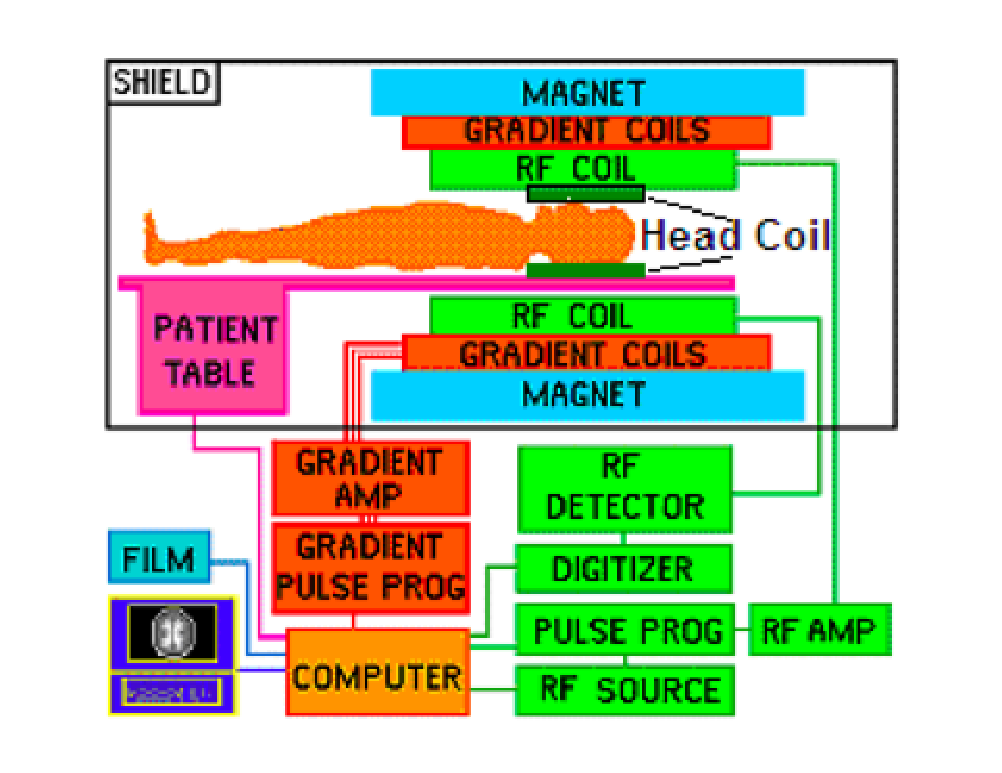
\includegraphics[width=4in]{background/images/MRI_hardware.eps}}}
  \end{minipage}
\caption{Simplified block diagram of a typical MRI scanner} \label{fig:scanner_block}
\end{figure}

\subsection{Physics of Signal Formation and Detection}

The signal source in MRI is the macroscopic magnetization produced by excited nuclear spins in the 
imaged object. Spin is a fundamental quantum property of elementary particles just like electrical 
charge or mass, which is related to the angular momentum of the nucleus. In classical terms, angular 
momentum is due to spinning of an object about its axis. Spin quantum numbers come discrete, i.e.,  in 
multiples of $\frac{1}{2}$, and can be either positive or negative. The total spin quantum number of 
$\frac{1}{2}$ paired protons
and neutrons equals zero, while unpaired protons and neutrons in a nucleus each contribute a spin 
quantum number of $\frac{1}{2}$. Thus, a nucleus with an uneven number of nucleons (protons or neutrons) 
has a nonzero spin quantum number, which is a multiple of $\frac{1}{2}$, 
and a large number of them can, therefore, 
produce a net magnetization when placed in an external magnetic field. The most abundant nucleus with 
uneven number of nucleons in the human body is hydrogen with just one proton.

In MRI, an ensemble of nuclei of the same type, such as hydrogen, present in an object being imaged is 
called a nuclear spin system. Although nuclear spin is a property of the individual nucleus, 
characterized by quantum mechanics, with the large number of nuclei present in bulk matter, the bulk 
behavior of a spin system can be described in classical physics terms and the macroscopic magnetization 
is no longer discrete.

A single nucleus with a nonzero spin, such as hydrogen, creates a small magnetic field, which is 
represented by the vector quantity $\mu$, called the nuclear magnetic moment. Spin angular momentum 
$\textbf{J}$ and magnetic moment are linearly related to each other by

\begin{equation}
  \mu = \frac{\gamma}{2}\pi J
\end{equation}

which $\gamma$ is gyromagnetic ratio.

\subsection{Distortion Origin and Manifestations}

Spatial indexing in MRI is accomplished by gradient coils in three orthogonal directions. In image 
reconstruction, gradients are assumed linear throughout the imaging volume. Due to pragmatic 
constraints, further considered below, it is difficult to achieve this situation.

For a patient to fit comfortably, the bore of the main magnet must be as large as possible. The larger 
the bore, the more difficult it is to generate a linear gradient. In general, the gradient along the 
axis of the main magnet (z axis) has the highest linearity compared to the other two directions 
(x and y) due to physical constraints.

Consider a slice of constant z, read in x direction. In the slice image, gradient field non-linearity 
distortion manifests itself in two ways. First, due to non-linearities in the x gradient, $G_x$, and in 
the y-gradient, $G_y$, there is a systematic transverse distortion in the slice plane. Second, 
because of 
the gradient field non-linearity, a potato chip effect takes place along the slice selection direction 
(z). Although MRI slices are usually considered to be planes, in actuality, because of gradient field 
non-linearity, these planes tend to warp into a “potato chip-like” shapes. This distortion is difficult
to correct in 2D imaging but can be, in principle, corrected in 3D imaging methods.

\subsection{The Gradient Coils}

Misregistration caused by gradient field non-linearities occur in all three directions. The magnetic 
fields generated by the three gradient coils and the main magnet lie along the z-axis.  Due to the 
strength of the main B0 field, any other component of the gradient fields can be neglected. 

The z-gradient coil is designed to produce a linear variation in the z-component of the field along the
axis of the magnet, with a high degree of gradient uniformity in the transverse plane. Circular wire 
loops are the most obvious choice since they are azimuthally symmetric and possess reasonable radial 
uniformity. Since the gradient fields have to be symmetric with respect to the gradient isocenter, the 
coils are usually arranged as pairs. For the z-gradient, the current in the coil pair, called Maxwell 
pair, is equal in magnitude, but opposite in direction (see Fig. ~\ref{fig:coil_axis} (a)). 
Coils on one side of the z = 0 
plane generate fields parallel to B0 while fields due coils on the other side are anti-parallel to 
$B_0$ 
leading to an overall field variation along z. The relation between the radius a of the coils and their
axial distance d is optimized in order to minimize all but the linear z-term in the polynomial 
expansion of the field described below.
 
\begin{figure}[htb]
  \begin{minipage}[b]{2.5in}
    \centering
    \centerline{\mbox{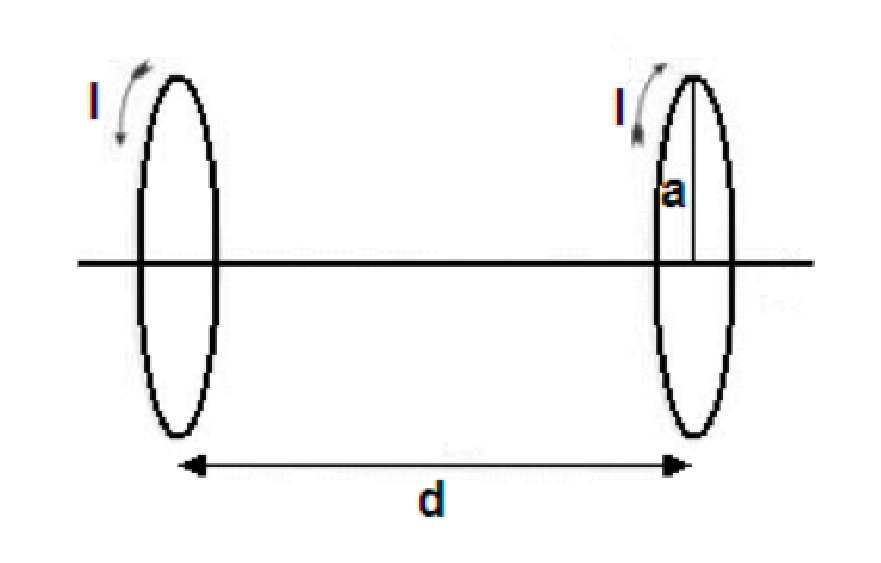
\includegraphics[width=2.5in]{background/images/coil_z.eps}}}
    \centerline{\mbox{\emph{(a)}}}
  \end{minipage}
  \begin{minipage}[b]{3in}
    \centering
    \centerline{\mbox{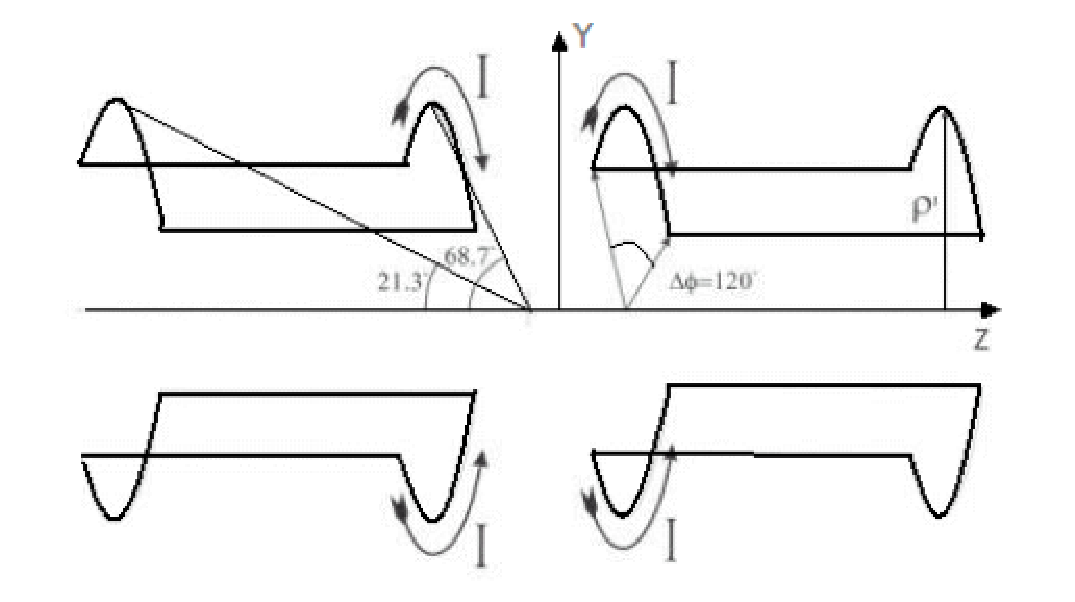
\includegraphics[width=3in]{background/images/coil_y.eps}}}
    \centerline{\mbox{\emph{(b)}}}
  \end{minipage}
  \caption{(a) Principal design of a Maxwell pair of coils generating the z-gradient field. (b) Golay arrangement of a coils producing a y-gradient. Note that the field direction coincides with the z axis.} 
  \label{fig:coil_axis}
\end{figure}

The design of the gradient coils in x and y-direction is more complicated. The principle design, called Golay arrangement, is shown in Fig. ~\ref{fig:coil_axis}(b). The x- and y-gradient coils are identical except for a rotation by 90 degrees. 

\subsection{Physical and Mathematical Description of Nonlinear Gradient Fields}

The following description of nonlinear gradient field was given by Dr. Sumanaweera in his thesis 
\cite{sumanaweera_thesis}. Let \textbf{B} the magnetic flux density and \textbf{H} be the magnetic field intensity vectors produced by any of the gradient coils. The relationship between these vector quantities is 
\begin{equation}
  \textbf{B} = \mu \textbf{H}
\end{equation}

where $\mu$ is the permeability of the medium. Gradient fields are usually quasistatic (slowly varying in time) magnetic fields, therefore, displacement currents in the medium inside the coil may be ignored unless very rapid sequences are used. Electromagnetic field theory tells us that a quasistatic magnetic field in a current free region can be described by a scalar magnetic field potential ψ such that 

\begin{equation}
  \textbf{H} = - \nabla \psi 
\end{equation}

A fundamental property of magnetic fields is that its divergence is always zero, thus $\nabla \cdot \mathbf{B} = 0$ everywhere, and therefore the scalar magnetic potential satisfies Laplace’s equation:
\begin{equation}
  \nabla^2 \psi = 0 
\end{equation}

It can be shown that solutions of Laplace’s equation can be expressed as linear combinations of 
homogeneous polynomials  in the coordinates x, y, z. In order to describe the nonlinearity of a 
gradient field, one usually decomposes the field into the ideal linear term and additional nonlinear 
field terms; the latter are expanded into homogenous polynomials. Furthermore, if one assumes circular 
symmetry, which means that there is no specific angular dependence of the nonlinear field terms, one 
obtains following general expressions for the three gradient fields $B_x$, $B_y$, and $B_z$

\begin{align}
  B_x &= G_x x \left[ 1 + \sum^{\infty}_{i=1}A_i\sum^{i}_{j=0}a_jz^{2(i-j)}(x^2 + y^2)^j \right] \nonumber \\
  B_y &= G_y y \left[ 1 + \sum^{\infty}_{i=1}B_i\sum^{i}_{j=0}b_jz^{2(i-j)}(x^2 + y^2)^j \right] \label{eqn:distortion1}\\
  B_z &= G_c z \left[ 1 + \sum^{\infty}_{i=1}C_i\sum^{i}_{j=0}c_jz^{2(i-j)}(x^2 + y^2)^j \right] \nonumber 
\end{align}

Note that if the nonlinear terms vanish, the gradient fields become perfectly linear. In general, the higher order polynomials in these field equations are insignificant (contribute very little to the field) and can therefore be ignored. In practice, it is sufficient to include only polynomials up to the second order $i = 2$ in $x^2$, $y^2$, and $z^2$. Thus, the field gradient expressions become:

\begin{align}
  B_x &\cong G_x x \left[ 1 + K_{x0}(x^2 + y^2) + K_{x1}z^2 + K_{x2}z^2(x^2 + y^2) + \right. \nonumber \\
      &\qquad \left. K_{x3}(x^2 + y^2)^2 + K_{x4}z^4 \right] \nonumber \\
  B_y &\cong G_y y \left[ 1 + K_{y0}(x^2 + y^2) + K_{y1}z^2 + K_{y2}z^2(x^2 + y^2) + \right. \nonumber \\
      &\qquad \left. K_{y3}(x^2 + y^2)^2 + K_{y4}z^4 \right] \label{eqn:distortion2}\\
  B_z &\cong G_c z \left[ 1 + K_{z0}(x^2 + y^2) + K_{z1}z^2 + K_{z2}z^2(x^2 + y^2) + \right. \nonumber \\
      &\qquad \left. K_{z3}(x^2 + y^2)^2 + K_{z4}z^4 \right] \nonumber
\end{align}

where we have introduced new constants K (for example, $K_{x0} = A_0 a_0$). Since the coordinate distortion function can be expressed as:
\begin{equation}
  x' = x(1 + \nabla G_x) \equiv f_x(x)
\end{equation}

we have: 
\begin{align}
  f(x) &= x \left[ 1 + K_{x0}(x^2 + y^2) + K_{x1}z^2 + K_{x2}z^2(x^2 + y^2) + \right. \nonumber \\
  &\qquad \left. K_{x3}(x^2 + y^2)^2 + K_{x4}z^4 \right] \nonumber \\
  f(y) &= G_y y \left[ 1 + K_{y0}(x^2 + y^2) + K_{y1}z^2 + K_{y2}z^2(x^2 + y^2) + \right. \nonumber \\
      &\qquad \left. K_{y3}(x^2 + y^2)^2 + K_{y4}z^4 \right] \label{eqn:distortion3} \\
  f(z) &= G_c z \left[ 1 + K_{z0}(x^2 + y^2) + K_{z1}z^2 + K_{z2}z^2(x^2 + y^2) + \right. \nonumber \\
      &\qquad \left. K_{z3}(x^2 + y^2)^2 + K_{z4}z^4 \right] \nonumber
\end{align}

Equation ~\ref{eqn:distortion3} can be conveniently written in matrix form as

\begin{equation}
  r' = r + K \cdot F(r)
\end{equation}

where $r'$ is the distorted coordinate vector derived from the undistorted vector $r$, $K$ is the distortion parameter matrix formed by the elements $K_{α,i}$ , $\alpha = x, y, z, i = 0,1,\cdots 4$, and $F(r)$ is a nonlinear six-dimensional vector field given by
\begin{equation}
  F(r) = 
  \begin{bmatrix}
    x(x^2 + y^2) \\
    xz^2 \\
    xz^2(x^2 + y^2) \\
    x(x^2 + y^2)^2 \\
    z^4 \\
  \end{bmatrix} 
\end{equation}

% \section{Previous Work}

% Previous study was conducted using a 159.50mm × 159.70mm × 158.11mm oil phantom inside a 1.5 Tesla(T) 
% MRI scanner as shown in figure 

% \begin{figure}[htb]
%   \begin{minipage}[b]{2.75in}
%     \centering
%     \centerline{\mbox{\includegraphics[width=2.75in]{background/images}
    
%   \end{minipage}
% \end{figure}

% \begin{enumerate}
%   \item Magnetic Resonance Imaging
    
%   \item mri distortion
%   \item previous work in mri distortion correction (mention tom's thesis and work before that)
% \end{enumerate}
